<<<<<<< HEAD
% Created 2024-10-27 Sun 21:59
=======
% Created 2024-10-20 Sun 21:02
>>>>>>> 26a94091299b2cda35efc4a2f640ed92afe36773
% Intended LaTeX compiler: lualatex
\documentclass[presentation,professionalfonts,aspectratio=169]{beamer}
                

% 
\makeatletter
 \@ifclassloaded{beamer}{%
  %%% save beamer's `solution' environment as `beamersolution':
  \let\beamersolution\solution
  \let\endbeamersolution\endsolution
  %%% "delete" the `solution' environment:
  \let\solution\relax
  \let\endsolution\relax
}{%
}%
\makeatother
\usepackage[utf8]{inputenc}
\usepackage[T1]{fontenc}
%\usepackage[french]{babel}
\usepackage[portuguese]{babel}

%%%% FONTS




\usepackage{xsim}
\usepackage[most]{tcolorbox}
\usepackage{amssymb}
\usepackage{fontawesome}
\newcounter{paragraph}



\DeclareExerciseEnvironmentTemplate{custom}{%
  \begin{tcolorbox}[boxrule = 0pt]
  \tcbox[on line,colback=teal,colframe=teal,coltext=white,size=small]{%
    \faBook\sffamily\bfseries\
    \XSIMmixedcase{\GetExerciseName}
    \GetExerciseProperty{counter}%
  }\quad
}{\end{tcolorbox}}


\DeclareExerciseEnvironmentTemplate{custom2}{%
  \begin{tcolorbox}[boxrule = 0pt]
  \tcbox[on line,colback=violet,colframe=violet,coltext=white,size=small]{%
    \faToggleOn\sffamily\bfseries\
    \XSIMmixedcase{\GetExerciseName}
    \GetExerciseProperty{counter}%
  }\quad
}{\end{tcolorbox}}




\DeclareExerciseType{test}{
	exercise-env = question ,
	solution-env = answer ,
	exercise-template = custom ,
	solution-template = custom2 ,
	exercise-name	= Exemplo. ,
	exercises-name = Exemplo ,
	solution-name = Solução ,
	solutions-name = Sol. ,
	exercise-heading = \textbf ,
	solution-heading = \textbf
}


\xsimsetup{
  exercise/within = section,
  exercise/the-counter =  \arabic{exercise}, 
%%solution-name = solution,  % used with headings=true
solution/print=false,
%print-collection/print=both,
}





\usepackage{colortbl}
\usepackage[tikz]{bclogo}
\usetikzlibrary{fit,patterns,shadows.blur,shapes,mindmap}
\usetikzlibrary{arrows,calc,arrows.meta,decorations.markings,shapes.symbols}
\usetikzlibrary{decorations.pathreplacing, decorations.pathmorphing,calc,arrows,positioning}
\usepackage{tikzpeople}
\usepackage{qrcode,hyperref}
\usepackage{upgreek}
%\usepackage[version=4]{mhchem}
\usepackage{tabularray}


\NewTblrTheme{fancy}{
\SetTblrStyle{caption-tag}{font=\bfseries}
\SetTblrInner[tblr,longtblr]{rowsep=2.5pt}
\DefTblrTemplate{firsthead, middlehead,lasthead}{default}{} % <---
\DefTblrTemplate{contfoot-text}{normal}{\scriptsize\textit{Continued on the next page}}
\SetTblrTemplate{contfoot-text}{normal}
}






\usepackage{chemfig,chemmacros,elements,chemformula}
\chemsetup{modules={all}}
\chemsetup[redox]{pos=top,roman=false}
\chemsetup[redox]{pos=top}
\chemsetup{redox/sep=.5em}
\chemsetup[redox]{explicit-sign=true}
\NewChemPhase\lqdd{\(\ell\)}
\NewChemPhase\gr{grafite}
\NewChemPhase\reac{reação}
\NewChemState\Enthalpy{symbol=H,superscript=,unit=\kilo\joule}%
\usepackage{siunitx}
\setchemfig{fixed length=false, atom sep=2.5em, arrow offset=6pt, scheme debug=false}%,angle increment=30}
\renewcommand*\printatom[1]{\ensuremath{\mathsf{#1}}} % This line changes the font of the atoms to sans serif
%%%% QRCODE
\usepackage{pdfpages}
\usepackage{mol2chemfig}
\usepackage{subfig,caption}
\usepackage{wrapfig}
\usepackage{enumitem}
\setitemize{label=\usebeamerfont*{itemize item}%
\usebeamercolor[fg]{itemize item}
\usebeamertemplate {itemize item}}
\usepackage{array} % ajust colunm table
\usepackage{cancel}
\usepackage[controls]{animate}
\renewcommand{\CancelColor}{\color{red}}

%%%%%%%%%%%%%%%%%%% CONFIG TCOLORBOX 

\newtcolorbox{mybox}[2][]{boxsep=0.5em,left=0.5em,
colback=blue!5!white, colframe=blue!75!black,
fonttitle=\bfseries\sffamily,
colbacktitle=blue!85!red!60,enhanced,
attach boxed title to top left={yshift=-3mm,xshift=5mm},
title=#2,#1}

\newtcolorbox{myrule}[2][]{boxsep=0.5em,left=0.5em,
colback=green!5!white, colframe=blue!75!black,
fonttitle=\bfseries\sffamily,
colbacktitle=blue!85!red!60,enhanced,
attach boxed title to top left={yshift=-3mm,xshift=5mm},
title=#2,#1}


\newtcolorbox{myex}[2][]{boxsep=0.5em,left=0.5em,
  colback=yellow!5!white, colframe=blue!75!black, 
  fonttitle=\bfseries\sffamily,
  colbacktitle=blue!85!red!60,enhanced,
  attach boxed title to top left={yshift=-3mm,xshift=5mm},
  title=#2,#1}


 \definecolor{col1}{HTML}{FF7878}
 \definecolor{col2}{HTML}{51B5F8}
 \definecolor{col3}{HTML}{68E1AA}
 \definecolor{col4}{HTML}{B869EA}
 \definecolor{col5}{HTML}{FF5500}
 \definecolor{col6}{HTML}{FFF8E7}
 \definecolor{col7}{HTML}{FF9966}
 \definecolor{col8}{HTML}{9400D3}



\definesubmol\nobond{-[,0.2,,,draw=none]\scriptstyle\color{blue}}
\newcommand{\re}{\hspace{-1cm}}
\newcommand{\af}{\hspace{2cm}}

%%%% Config X sim for BEAMER
\usepackage{ragged2e}
\justifying
\makeatletter
\@ifclassloaded{beamer}{%
%%% save beamer's `solution' environment as `beamersolution':
\let\beamersolution\solution
\let\endbeamersolution\endsolution
%%% "delete" the `solution' environment:
\let\solution\relax
\let\endsolution\relax
}{%
}%
\makeatother
\usepackage[utf8]{inputenc}
\usepackage[T1]{fontenc}
%\usepackage[portuguese, ]{babel}
%%%% FONTS
%%% XSIM CONFIG BEAMER
\usepackage{xsim}
\usepackage{amsmath}
\usepackage[most]{tcolorbox}
\usepackage{amssymb}
\usepackage{fontawesome}
\usepackage{tasks}
\newcounter{paragraph}
%\usepackage[dvipsnames,svgnames]{xcolor}
\usepackage{xcolor}
\usepackage{annotate-equations}
%%% BOX EXERCISE BEAMER
\DeclareExerciseEnvironmentTemplate{custom}{%
\begin{tcolorbox}[boxrule = 0pt]
\tcbox[on line,colback=teal,colframe=teal,coltext=white,size=small]{%
\faBook\sffamily\bfseries\
\XSIMmixedcase{\GetExerciseName}
\GetExerciseProperty{counter}%
}\quad
}{\end{tcolorbox}}
%% == CUSTOM BOX BEAMER
\DeclareExerciseEnvironmentTemplate{custom2}{%
\begin{tcolorbox}[boxrule = 0pt]
\tcbox[on line,colback=violet,colframe=violet,coltext=white,size=small]{%
\faToggleOn\sffamily\bfseries\
\XSIMmixedcase{\GetExerciseName}
\GetExerciseProperty{counter}%
}\quad
}{\end{tcolorbox}}
\DeclareExerciseType{test}{
exercise-env = question ,
solution-env = answer ,
exercise-template = custom ,
solution-template = custom2 ,
exercise-name = Exemplo ,
exercises-name = Exemplo ,
solution-name = Solução ,
solutions-name = Sol. ,
exercise-heading = \textbf ,
solution-heading = \textbf
}
\xsimsetup{
exercise/within = section,
exercise/the-counter =  \arabic{exercise},
%%solution-name = solution,  % used with headings=true
solution/print=true,
print-collection/print=both,
}
\NewTasksEnvironment[label = (\emph{\alph*}),
label-width = 12pt]{choice}[\choice]
\usepackage{empheq} %%% Brackers
\usepackage{colortbl}
\usepackage[tikz]{bclogo}
\usetikzlibrary{fit,patterns,shadows.blur,shapes,mindmap}
\usetikzlibrary{arrows,arrows.meta,decorations.markings,shapes.symbols}
\usetikzlibrary{decorations.pathreplacing, decorations.pathmorphing,calc,arrows,positioning,snakes}
\usepackage{tikzpeople}
\usepackage{qrcode,hyperref}
\usepackage{upgreek}
%\usepackage[version=4]{mhchem}
\usepackage{tabularray}
%%% PACKAGE PLOT GRAPH
\usepackage{pgfplots}
\pgfplotsset{width=10cm,compat=1.9}
%%% CUSTOM TABLE
\NewTblrTheme{fancy}{
\SetTblrStyle{caption-tag}{font=\bfseries,red2}
\SetTblrInner[tblr,longtblr]{rowsep=2.5pt}
\DefTblrTemplate{firsthead, middlehead,lasthead}{default}{} % <---
\DefTblrTemplate{contfoot-text}{normal}{\scriptsize\textit{Continua ...}}
\SetTblrTemplate{contfoot-text}{normal}
}
%% ==== CHEMMACROS E CHEMFIG CONFIG
\usepackage{chemfig,chemmacros,elements,chemformula}
\chemsetup{modules={all}}
\chemsetup[redox]{pos=top,roman=false}
\chemsetup[redox]{pos=top}
\chemsetup{redox/sep=.5em}
\chemsetup[redox]{explicit-sign=true} %%% reaction redox
%% == CUSTOM PHASES IN CHEMMACROS
\NewChemPhase\lqdd{\(\ell\)}
\NewChemPhase\gr{grafite}
\NewChemPhase\reac{reação}
\NewChemState\Enthalpy{symbol=H,superscript=,unit=\kilo\joule}%
\usepackage{siunitx}
\setchemfig{fixed length=false, atom sep=2.5em, arrow offset=6pt, scheme debug=false}
%% == NUMEROS PARA FORMULES
\renewcommand*\printatom[1]{\ensuremath{\mathsf{#1}}} % This line changes the font of the atoms to sans serif
%%% INCLUDE PAGES PDFs
\usepackage{pdfpages}
\usepackage{mol2chemfig}
\usepackage{subfig,caption}
\usepackage{wrapfig}
\usepackage{enumitem}
\setitemize{label=\usebeamerfont*{itemize item}%
\usebeamercolor[fg]{itemize item}
\usebeamertemplate {itemize item}}
\usepackage{array} % ajust colunm table
\usepackage{cancel}
\usepackage[controls]{animate}
\renewcommand{\CancelColor}{\color{red}}
%%%%%%%%%%%%%%%%%%% CONFIG TCOLORBOX
\newtcolorbox{mybox}[2][]{boxsep=0.5em,left=0.5em,
colback=blue!5!white, colframe=blue!75!black,
fonttitle=\bfseries\sffamily,
colbacktitle=blue!85!red!60,enhanced,
attach boxed title to top left={yshift=-3mm,xshift=5mm},
title=#2,#1}
\newtcolorbox{myrule}[2][]{boxsep=0.5em,left=0.5em,
colback=green!5!white, colframe=blue!75!black,
fonttitle=\bfseries\sffamily,
colbacktitle=blue!85!red!60,enhanced,
attach boxed title to top left={yshift=-3mm,xshift=5mm},
title=#2,#1}
\newtcolorbox{myex}[2][]{boxsep=0.5em,left=0.5em,
colback=yellow!5!white, colframe=blue!75!black,
fonttitle=\bfseries\sffamily,
colbacktitle=blue!85!red!60,enhanced,
attach boxed title to top left={yshift=-3mm,xshift=5mm},
title=#2,#1}
\tcbset{colback=yellow!10!white, colframe=red!50!black, highlight math style= {enhanced, %<-- needed for the ’remember’ options
colframe=red,colback=red!10!white,boxsep=0pt}}
\definecolor{col1}{HTML}{FF7878}
\definecolor{col2}{HTML}{51B5F8}
\definecolor{col3}{HTML}{68E1AA}
\definecolor{col4}{HTML}{B869EA}
\definecolor{col5}{HTML}{FF5500}
\definecolor{col6}{HTML}{FFF8E7}
\definecolor{col7}{HTML}{FF9966}
\definecolor{col8}{HTML}{9400D3}
%% CONFIG COLOR CARBONO
\tikzstyle{bal}=[inner sep=0.3pt,fill=orange,fill opacity=0.5,circle,minimum size=0.2cm]
\tikzstyle{rect}=[inner sep=0.3pt,fill=red,fill opacity=0.5,circle,minimum size=0.2cm]
\tikzstyle{bal2}=[inner sep=0.3pt,fill=blue,fill opacity=0.5,circle,minimum size=0.2cm]
\tikzstyle{bal3}=[inner sep=0.3pt,fill=yellow,fill opacity=0.5,circle,minimum size=0.2cm]
\definesubmol\nobond{-[,0.2,,,draw=none]\scriptstyle\color{blue}}
\newcommand{\re}{\hspace{-1cm}}
\newcommand{\af}{\hspace{2cm}}
\tikzstyle{mybox} = [draw=red, fill=blue!20, very thick, rectangle, rounded corners, inner sep=10pt, inner ysep=20pt]
\tikzstyle{fancytitle} =[fill=red, text=white]
\date{}
%\usetheme{minflat}
\DeclareExerciseCollection{Concentracoes}
\usetheme{minflat}
\author{Fábio Lima}
\date{}
\title{ Soluções}
\hypersetup{
 pdfauthor={Fábio Lima},
 pdftitle={ Soluções},
 pdfkeywords={},
 pdfsubject={},
 pdfcreator={Emacs 29.4 (Org mode 9.6.15)}, 
 pdflang={En Portuguese}}
\begin{document}

\begingroup
  \setbeamertemplate{headline}{}
  \maketitle
  \endgroup
\begin{frame}{Sumário}
\tableofcontents
\end{frame}


<<<<<<< HEAD

\section{Soluções}
\label{sec:orge930067}

\begin{frame}[label={sec:orgbd3cab3}]{Soluções}
\begin{description}
\item[{Solução:}] é uma mistura homogênea de soluto e solvente
\item[{Solvente:}] Componente cujo estado físico é preservado.
\item[{Soluto:}] Dissolvido no solvente

=======
\section{Soluções}
\label{sec:org5ece32a}

\begin{frame}[label={sec:orgab80f7e}]{Soluções}
\begin{description}
\item[{Solução:}] é uma mistura homogênea de soluto e solvente
\item[{Solvente:}] Componente cujo estado físico é preservado.
\item[{Soluto:}] Dissolvido no solvente

>>>>>>> 26a94091299b2cda35efc4a2f640ed92afe36773
\alert{Observação:} \emph{Se todos os componentes estiverem no mesmo estado físico, o solvente é aquele presente em maior quantidade.}
\end{description}
\end{frame}

<<<<<<< HEAD
\begin{frame}[label={sec:org3015545}]{Solubilidade \emph{versus} Temperatura}
=======
\begin{frame}[label={sec:orgeb2cd50}]{Solubilidade \emph{versus} Temperatura}
>>>>>>> 26a94091299b2cda35efc4a2f640ed92afe36773
\begin{columns}
\begin{column}{0.4\columnwidth}
\begin{figure}
\centering 
\begin{tikzpicture}[scale=0.5, transform shape]]
	\begin{axis}[
       ylabel=Solubilidade g/g \ch{H2O},
		xlabel=Temperatura / \si{\celsius},
		title=Curva de Solubilidade, 
		legend style={draw=none},
		legend pos=north west]
		%% KNO3
	\addplot[color=red,mark=*] coordinates {
		(0,13.25)
		(20,31.66)
		(40,63.9)
		(60,109.9)
		(80,169)
		(100,245.2)
	};
	%%% KI
	\addplot[color=blue,mark=*] coordinates {
		(0,127.8)
		(20,144.51)
		(40,161)
		(60,176.2)
		(80,191.5)
		(100,208)
	};
	%% KClO4
	\addplot[color=black,mark=*] coordinates {
		(0,0.76)
		(20,1.73)
		(40,3.63)
		(60,7.18)
		(80,13.38)
		(100,22.2)
	};
	%% NaCl
	%35.6	35.8	36.42	37.05	38.05	39.2
	\addplot[color=green,mark=*] coordinates {
		(0,35.6)
		(20,35.8)
		(40,36.42)
		(60,37.05)
		(80,38.05)
		(100,39.2)
	};
	\legend{\ch{KNO3}, KI, \ch{KC$\ell$O4}, \ch{NaC$\ell$}}
	\end{axis}
\end{tikzpicture}
\caption{Curvas de Solubilidade}
\end{figure}
\end{column}
<<<<<<< HEAD

\begin{column}{0.6\columnwidth}
\begin{itemize}
\item A solubilidade de uma substância é a quantidade máxima de uma substância que pode ser dissolvida em uma quantidade fixa de solvente a uma determinada temperatura.
\item A solubilidade de uma substância geralmente aumenta com a temperatura.
\item As moléculas da substância têm mais energia cinética a temperaturas mais altas, o que torna mais provável que elas colidam com as moléculas do solvente e se dissolvam.
\end{itemize}
\end{column}
\end{columns}
\end{frame}


\section{Concentrações}
\label{sec:orgd278599}



\begin{frame}[label={sec:org5f28868}]{Concentração Comum (g/L)}
\begin{itemize}
\item A quantidade de soluto dissolvido num dado volume de solução é denominada de concentração
\item É o quociente entre a massa do soluto e o volume da solução
\item Concentração comum é expressa em \alert{g/L} ou \alert{\unit{\gram\per\litre}}
\end{itemize}



\begin{tcolorbox}[ams equation]
\mathcal{C}=\frac{m}{V}
\end{tcolorbox}
\end{frame}

\begin{frame}[label={sec:org0c166e6}]{Exemplo}
\begin{question}
Qual a massa de cloreto de sódio (NaC\(\ell\)) necessária para preparar 250 mL de uma solução aquosa de concentração igual a 58,5 \unit{\gram\per\litre}.
\end{question}

\begin{answer}[print=true]
\begin{tcolorbox}[ams align*]
\mathcal{C}=& \frac{m_{soluto}}{V_{\text{solu\c{c}\~ao}}} \\
m_{soluto} = & \mathcal{C} \cdot V(mL)_{\text{solu\c{c}\~ao}}\\
m_{soluto}= &  58\;\unit{\gram\per\cancel\litre} \cdot 0,25\; \unit{\cancel\litre}\\
m_{soluto}= & 14,625\; \unit{\gram}
\end{tcolorbox}
\end{answer}
\end{frame}

\begin{frame}[label={sec:orgbd017e9}]{Concentração molar \(\mathcal{M}\) (mol/L)}
\begin{tcolorbox}[ams align]
\mathcal{M}=\frac{m_{\rm massa\; soluto}}{MM_{massa\;molar} \cdot V_{\text{ solu\c{c}\~ao}}}
\end{tcolorbox}

\begin{itemize}
\item Expressa o número de moles do soluto em 1L de solução, sua unidade é \alert{mol/L} ou \alert{\unit{\mole\per\liter}}.
\item A molaridade exprime também o número de milimoles (mmol ou \num{e-3} mol) de um soluto por mililitro (mL ou \num{e-3} L) de solução.
\end{itemize}

\begin{tcolorbox}[ams equation]
\mathcal{M}=\frac{n_{moles\; soluto}}{V_{\text{solu\c{c}\~ao}}} \Longrightarrow \mathcal{M}=\frac{n_{mmol\; soluto}}{V(mL)_{\text{solu\c{c}\~ao}}}
\end{tcolorbox}

\begin{itemize}
\item Se soubermos a massa do soluto e o volume de solução, podemos calcular a concentração molar.
\end{itemize}
\end{frame}

\begin{frame}[label={sec:org3d06f64}]{Exemplo}
\begin{question}
Encontrar a molaridade de uma solução aquosa que contém 2,30 g de álcool etílico (EtOH; \ch{C2H5OH}) (MM = 46,07 \unit{\gram\per\mole}) em 3,50 L.
\end{question}

\visible<1->{

\begin{answer}[print=true]
\begin{tcolorbox}[ams align*]
\mathcal{M}=& \frac{m_{\rm massa\; soluto}}{MM_{massa\;molar} \cdot V_{\text{ solu\c{c}\~ao}}}\\
\mathcal{M}=& \frac{2,3}{46,07\cdot 3,5}\\
\mathcal{M}=& 0,0143\; \unit{\mol\per\litre}
\end{tcolorbox}
\end{answer}
}
\end{frame}


\section{Percentual de uma solução}
\label{sec:org16fb2bd}


\begin{frame}[label={sec:org5d9b9a4}]{Relação massa x volume}
\begin{tcolorbox}[ams align]
\%(m/v)=\frac{m}{v_{total}}\cdot 100\% & \quad \text{massa por volume}\\
\%(m/m)= \frac{m}{m_{total}}\cdot 100\% & \quad \text{massa por massa total}\\
\%(v/v)= \frac{v}{v_{total}}\cdot 100\% & \quad \text{volume por volume}
\end{tcolorbox}
\end{frame}


\begin{frame}[label={sec:org7a8d27d}]{Exemplo I}
\begin{question}
Uma solução foi preparada pela dissolução de 40 gramas de açúcar em 960 gramas de água. Determine seu título e sua porcentagem em massa?
\end{question}

\begin{answer}[print=true]
O título em massa é calculado através da relação entre massa de soluto e massa da solução, ou seja, 40 g/1000 g = \alert{0,04}. Portanto, a porcentagem em massa de açúcar na solução é de \alert{4\%}.
\end{answer}
\end{frame}


\begin{frame}[label={sec:org9858bd1}]{Exemplo II}
\begin{question}
Descreva o procedimento para preparar uma solução de Ácido sulfúrico com concentração de 1 \unit{\mol\per\litre} em 1 L de solução com pureza de 98\%. Dados: MM (\ch{H2SO4})= 98 \unit{\gram\per\mol} d=1,84 g/cm\textsuperscript{3}.

\begin{center}
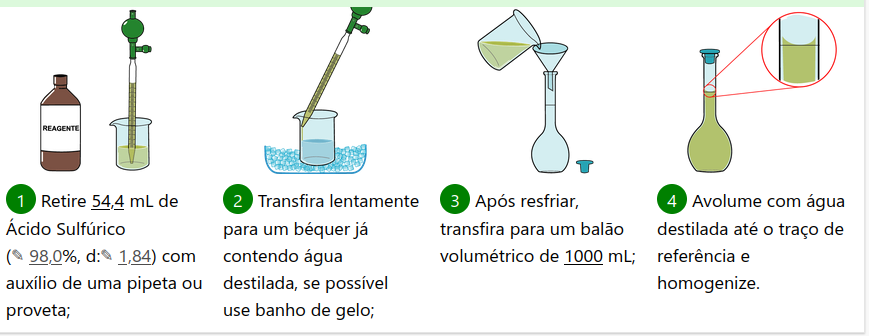
\includegraphics[scale=.3]{FQ/Solucoes/acid.png}
\end{center}
\end{question}
\end{frame}

\begin{frame}[label={sec:org9147d8a}]{}
\begin{answer}[print=true]
\scriptsize
\begin{description}
\item[{1:}] Estimar a massa do soluto
\end{description}
\begin{align*}
\mathcal{M}=\frac{m}{MM \cdot V} \Rightarrow 1 = \frac{m}{98 \cdot 1 } \Rightarrow m = 98 \; \text{g de}~ \ch{H2SO4}
\end{align*}
\begin{description}
\item[{2:}] Relacionar com densidade para achar o volume
\end{description}
\begin{align*}
\mathcal{d}=\frac{m}{v} \Rightarrow 1,84 ~\text{g/cm$^3$}=\frac{98}{v} \Rightarrow v=53,26 ~\text{mL}  
\end{align*}
\begin{description}
\item[{3:}] Relacione a pureza
\begin{align*}
& 53,26~\text{ mL} -\!\!\!-\!\!\!- 98~\text{\%}\\
& x~\text{mL} -\!\!\!-\!\!\!- 100~\text{\%}\\
& x= 54,4 ~\text{mL}
\end{align*}
\end{description}
\end{answer}
\end{frame}


\section{Partes por milhão e bilhão (ppm \& ppb)}
\label{sec:org8abc208}

\begin{frame}[label={sec:org5a2482e}]{Partes por milhão e bilhão (ppm \& ppb)}

\begin{tikzpicture}
	 \node[rectangle, draw = teal, text = white, fill = teal, minimum width = 2cm, minimum height = 1cm, font={\bfseries\large}] (r1) at (0,0) {PPM};
    \node[rectangle, draw = red, text = white, fill = red, minimum width = 2cm, minimum height = 1cm,
    font={\bfseries\large}] (r2) at (0,-1.5) {PPB};
        \node[rectangle, draw = gray, text = white, fill = gray, minimum width = 2cm, minimum height = 1cm,
    font={\bfseries\large}] (r3) at (0,-3.0) {PPT};
    \node[rectangle, draw=none, right=1cm of r1, font={\bfseries\Large}]{partes por milhão 1 mg/L};
    \node[rectangle, draw=none, right=1cm of r2, font={\bfseries\Large}]{partes por bilhão 1 $\mu$g/L};
    \node[rectangle, draw=none, right=1cm of r3, font={\bfseries\Large}]{partes por trilhão 1 ng/L};
\end{tikzpicture}


\begin{align*}
\text{ppm}=\frac{\text{massa soluto}}{\text{volume solução}} \times 10^6 & \Rightarrow  \frac{mg}{L}\\
\text{ppb}=\frac{\text{massa soluto}}{\text{volume solução}} \times 10^9 & \Rightarrow  \frac{\upmu g}{L}\\
\text{ppt}=\frac{\text{massa soluto}}{\text{volume solução}} \times 10^{12} & \Rightarrow  \frac{ng}{L}\\
\end{align*}
\end{frame}



\begin{frame}[label={sec:org761dc1a}]{Exemplo}
\begin{question}
\alert{(UFSCAR-SP)} O flúor tem um papel importante na prevenção e controle da cárie dentária. Estudos demonstram que, após a fluoretação da água, os índices de cáries nas populações têm diminuído. O flúor também é adicionado a produtos e materiais odontológicos. Suponha que o teor de flúor em determinada água de consumo seja 0,9 ppm (partes por milhão) em massa. Considerando a densidade da água 1g/mL, a quantidade, em miligramas, de flúor que um adulto ingere ao tomar 2 litros dessa água, durante um dia, é igual a

\begin{choice}(5)
\choice 0,09.
\choice 0,18.
\choice 0,90.
\choice 1,80.
\choice 18,0
\end{choice}
\end{question}
\end{frame}

\begin{frame}[label={sec:orge830c79}]{}
\begin{answer}[print=true]


Usar a densidade

\begin{align*}
d=\frac{m}{v} \Rightarrow 1 \text{g/mL}=\frac{m}{2000~\text{mL}} \Rightarrow  m = 2000 \; \text{g de \ch{H2O}}
\end{align*}

Cálculo da massa de flúor nesses 2 litros dessa água

\begin{align*}
\frac{0,9~g}{10^6~ \cancel{g}} \cdot 2000~\text{\cancel{g}} \Rightarrow 1,8 \times 10^{-3}~\text{g de F} 
\end{align*}

Isso corresponde a 1,8 mg de  flúor.
=======

\begin{column}{0.6\columnwidth}
\begin{itemize}
\item A solubilidade de uma substância é a quantidade máxima de uma substância que pode ser dissolvida em uma quantidade fixa de solvente a uma determinada temperatura.
\item A solubilidade de uma substância geralmente aumenta com a temperatura.
\item As moléculas da substância têm mais energia cinética a temperaturas mais altas, o que torna mais provável que elas colidam com as moléculas do solvente e se dissolvam.
\end{itemize}
\end{column}
\end{columns}
\end{frame}
\section{Densidade}
\label{sec:org2e0bdef}

\begin{frame}[label={sec:org2e43eee}]{Densidade (g/mL)}
\begin{itemize}
\item É a razão entre a massa da solução e o volume da solução.
\end{itemize}

\begin{tcolorbox}[ams equation]
\mathcal{d}=\frac{m_{\text{massa da solução}}}{V_{\text{solução}}}
\end{tcolorbox}

\begin{itemize}
\item Densidade da solução geralmente é expressa em \unit{\gram\per\ml} ou em \unit{\gram\per\cubic\centi\metre}. Nestes casos, para transformá-la em \unit{\gram\per\litre} deve-se multiplica-la por 1000.
\end{itemize}
\end{frame}


\section{Concentração Comum (g/L)}
\label{sec:org2708fee}

\begin{frame}[label={sec:org4e4d2a1}]{Concentração Comum (g/L)}
\begin{itemize}
\item A quantidade de soluto dissolvido num dado volume de solução é denominada de concentração
\item É o quociente entre a massa do soluto e o volume da solução
\item Concentração comum é expressa em \alert{g/L} ou \alert{g L\(^{-1}\)}

\begin{tcolorbox}[ams equation]
\mathcal{C}=\frac{m}{V}
\end{tcolorbox}
\end{itemize}
\end{frame}


\begin{frame}[label={sec:orgf8ee097}]{Exemplo}
\begin{question}
Qual a massa de cloreto de sódio (NaC\(\ell\)) necessária para preparar 250 mL de uma solução aquosa de concentração igual a 58,5 \unit{\gram\per\litre}.
\end{question}

\begin{answer}[print=true]
\begin{tcolorbox}[ams align*]
\mathcal{C}=& \frac{m_{soluto}}{V_{\text{solu\c{c}\~ao}}} \\
m_{soluto} = & \mathcal{C} \cdot V(mL)_{\text{solu\c{c}\~ao}}\\
m_{soluto}= &  58\;\unit{\gram\per\cancel\litre} \cdot 0,25\; \unit{\cancel\litre}\\
m_{soluto}= & 14,625\; \unit{\gram}
\end{tcolorbox}
>>>>>>> 26a94091299b2cda35efc4a2f640ed92afe36773
\end{answer}
\end{frame}


<<<<<<< HEAD

\section{Diluição de Soluções}
\label{sec:org4a5d702}


\begin{frame}[label={sec:orgc802ffa}]{Diluição de Soluções}
=======
\section{Concentração molar \(\mathcal{M}\) (mol/L)}
\label{sec:org69253a1}

\begin{frame}[label={sec:org992c6d6}]{Concentração molar \(\mathcal{M}\) (mol/L)}
\begin{itemize}
\item Expressa o número de moles do soluto em 1L de solução, sua unidade é \alert{mol/L} ou \alert{\unit{\mole\per\liter}}.
\item A molaridade exprime também o número de milimoles (mmol ou \num{e-3} mol) de um soluto por mililitro (mL ou \num{e-3} L) de solução.

\begin{tcolorbox}[ams equation]
\mathcal{M}=\frac{n_{moles\; soluto}}{V_{\text{solu\c{c}\~ao}}} \Longrightarrow \mathcal{M}=\frac{n_{mmol\; soluto}}{V(mL)_{\text{solu\c{c}\~ao}}}
\end{tcolorbox}

\item Se soubermos a massa do soluto e o volume de solução, podemos calcular a concentração molar.
\end{itemize}

\begin{tcolorbox}[ams align]
\mathcal{M}=\frac{m_{\rm massa\; soluto}}{MM_{massa\;molar} \cdot V_{\text{ solu\c{c}\~ao}}}
\end{tcolorbox}
\end{frame}

\begin{frame}[label={sec:orge768519}]{Exemplo}
\begin{question}
Encontrar a molaridade de uma solução aquosa que contém 2,30 g de álcool
etílico (EtOH; \ch{C2H5OH}) (MM = 46,07 \unit{\gram\per\mole}) em 3,50 L.
\end{question}

\visible<1->{

\begin{answer}[print=true]
\begin{tcolorbox}[ams align*]
\mathcal{M}=& \frac{m_{\rm massa\; soluto}}{MM_{massa\;molar} \cdot V_{\text{ solu\c{c}\~ao}}}\\
\mathcal{M}=& \frac{2,3}{46,07\cdot 3,5}\\
\mathcal{M}=& 0,0143\; \unit{\mol\per\litre}
\end{tcolorbox}
\end{answer}
}
\end{frame}


\section{Concentração de íons}
\label{sec:org4ba41a0}

\begin{frame}[label={sec:orgc63cdda}]{Concentração de íons}
\begin{itemize}
\item Conhecendo-se a molaridade de uma solução aquosa de um soluto que sofre ionização ou dissociação iônica, pode-se calcular as molaridade dos íons presentes na referida solução.
\end{itemize}

\begin{bclogo}[couleur=yellow!30 , arrondi=0.1 , logo=\bcplume , epBarre=3.5]{Equação de dissociação}


\begin{reactions*}
NaBr -> Na^+ + Br^- \\
MgF2 -> Mg^{+2} + 2 F^-\\
A$\ell$2S3 -> 2 A$\ell$^{+3} + 3 S^{-2}
\end{reactions*}
\end{bclogo}
\end{frame}

\begin{frame}[label={sec:orge441f2d}]{Exemplo}
\begin{question}
\small
Determine as concentrações molares dos íons  \ch{Ca^{+2}} e \ch{C$\ell$^-} presentes em uma solução aquosa 0,5 \unit{\mol\per\litre} de cloreto de cálcio, sabendo-se que este sal está 100\% dissociado.
\end{question}

\begin{answer}[print=true]
\scriptsize
\begin{reactions*}
1 CaC$\ell$2 & -> & 1 Ca^{+2} &\qquad  \;  +  & 2 C$\ell$^-\\
1 mol & & 1 mol & & 2 mols
\end{reactions*}

Na dissociação do cloreto de cálcio, observamos que 1 mol de \ch{CaC$\ell$2} fornece 1 mol de  \ch{Ca^{+2}} e 2 mols de \ch{C$\ell$^-}. Sendo a solução de \ch{CaC$\ell$2} 0,5 molar, conclui-se que as molaridades dos íons são:


\begin{reactions*}
1 CaC$\ell$2 & -> & 1 Ca^{+2} &\qquad \;  +  & 2 C$\ell$^-\\
0,5 \unit{\mol\per\litre} & & 0,5 \unit{\mol\per\litre} & & 1,0 \unit{\mol\per\litre}
\end{reactions*}
\end{answer}
\end{frame}


\section{Relação massa x volume}
\label{sec:org8fb1ad9}

\begin{frame}[label={sec:orga443b57}]{Relação massa x volume}
\begin{tcolorbox}[ams align]
\%(m/v)=\frac{m}{v_{total}}\cdot 100\% & \quad \text{massa por volume}\\
\%(m/m)= \frac{m}{m_{total}}\cdot 100\% & \quad \text{massa por massa total}\\
\%(v/v)= \frac{v}{v_{total}}\cdot 100\% & \quad \text{volume por volume}
\end{tcolorbox}
\end{frame}


\section{Diluição de Soluções}
\label{sec:org20444e1}
\begin{frame}[label={sec:orgfc9a2c7}]{Diluição de Soluções}
>>>>>>> 26a94091299b2cda35efc4a2f640ed92afe36773
\begin{itemize}
\item As soluções concentradas também podem ser misturadas com solventes para torná-las diluídas.
\item Em diluições a quantidade de solvente é que aumenta e a quantidade de soluto permanece sempre constante. Assim, o número inicial de mols do soluto é igual ao número de mols do soluto no final.mols do soluto no final.
\end{itemize}

\begin{tcolorbox}[ams align]
\mathcal{M}_1 \cdot V_1 = \mathcal{M}_2 \cdot V_2 
\end{tcolorbox}

<<<<<<< HEAD

\begin{center}
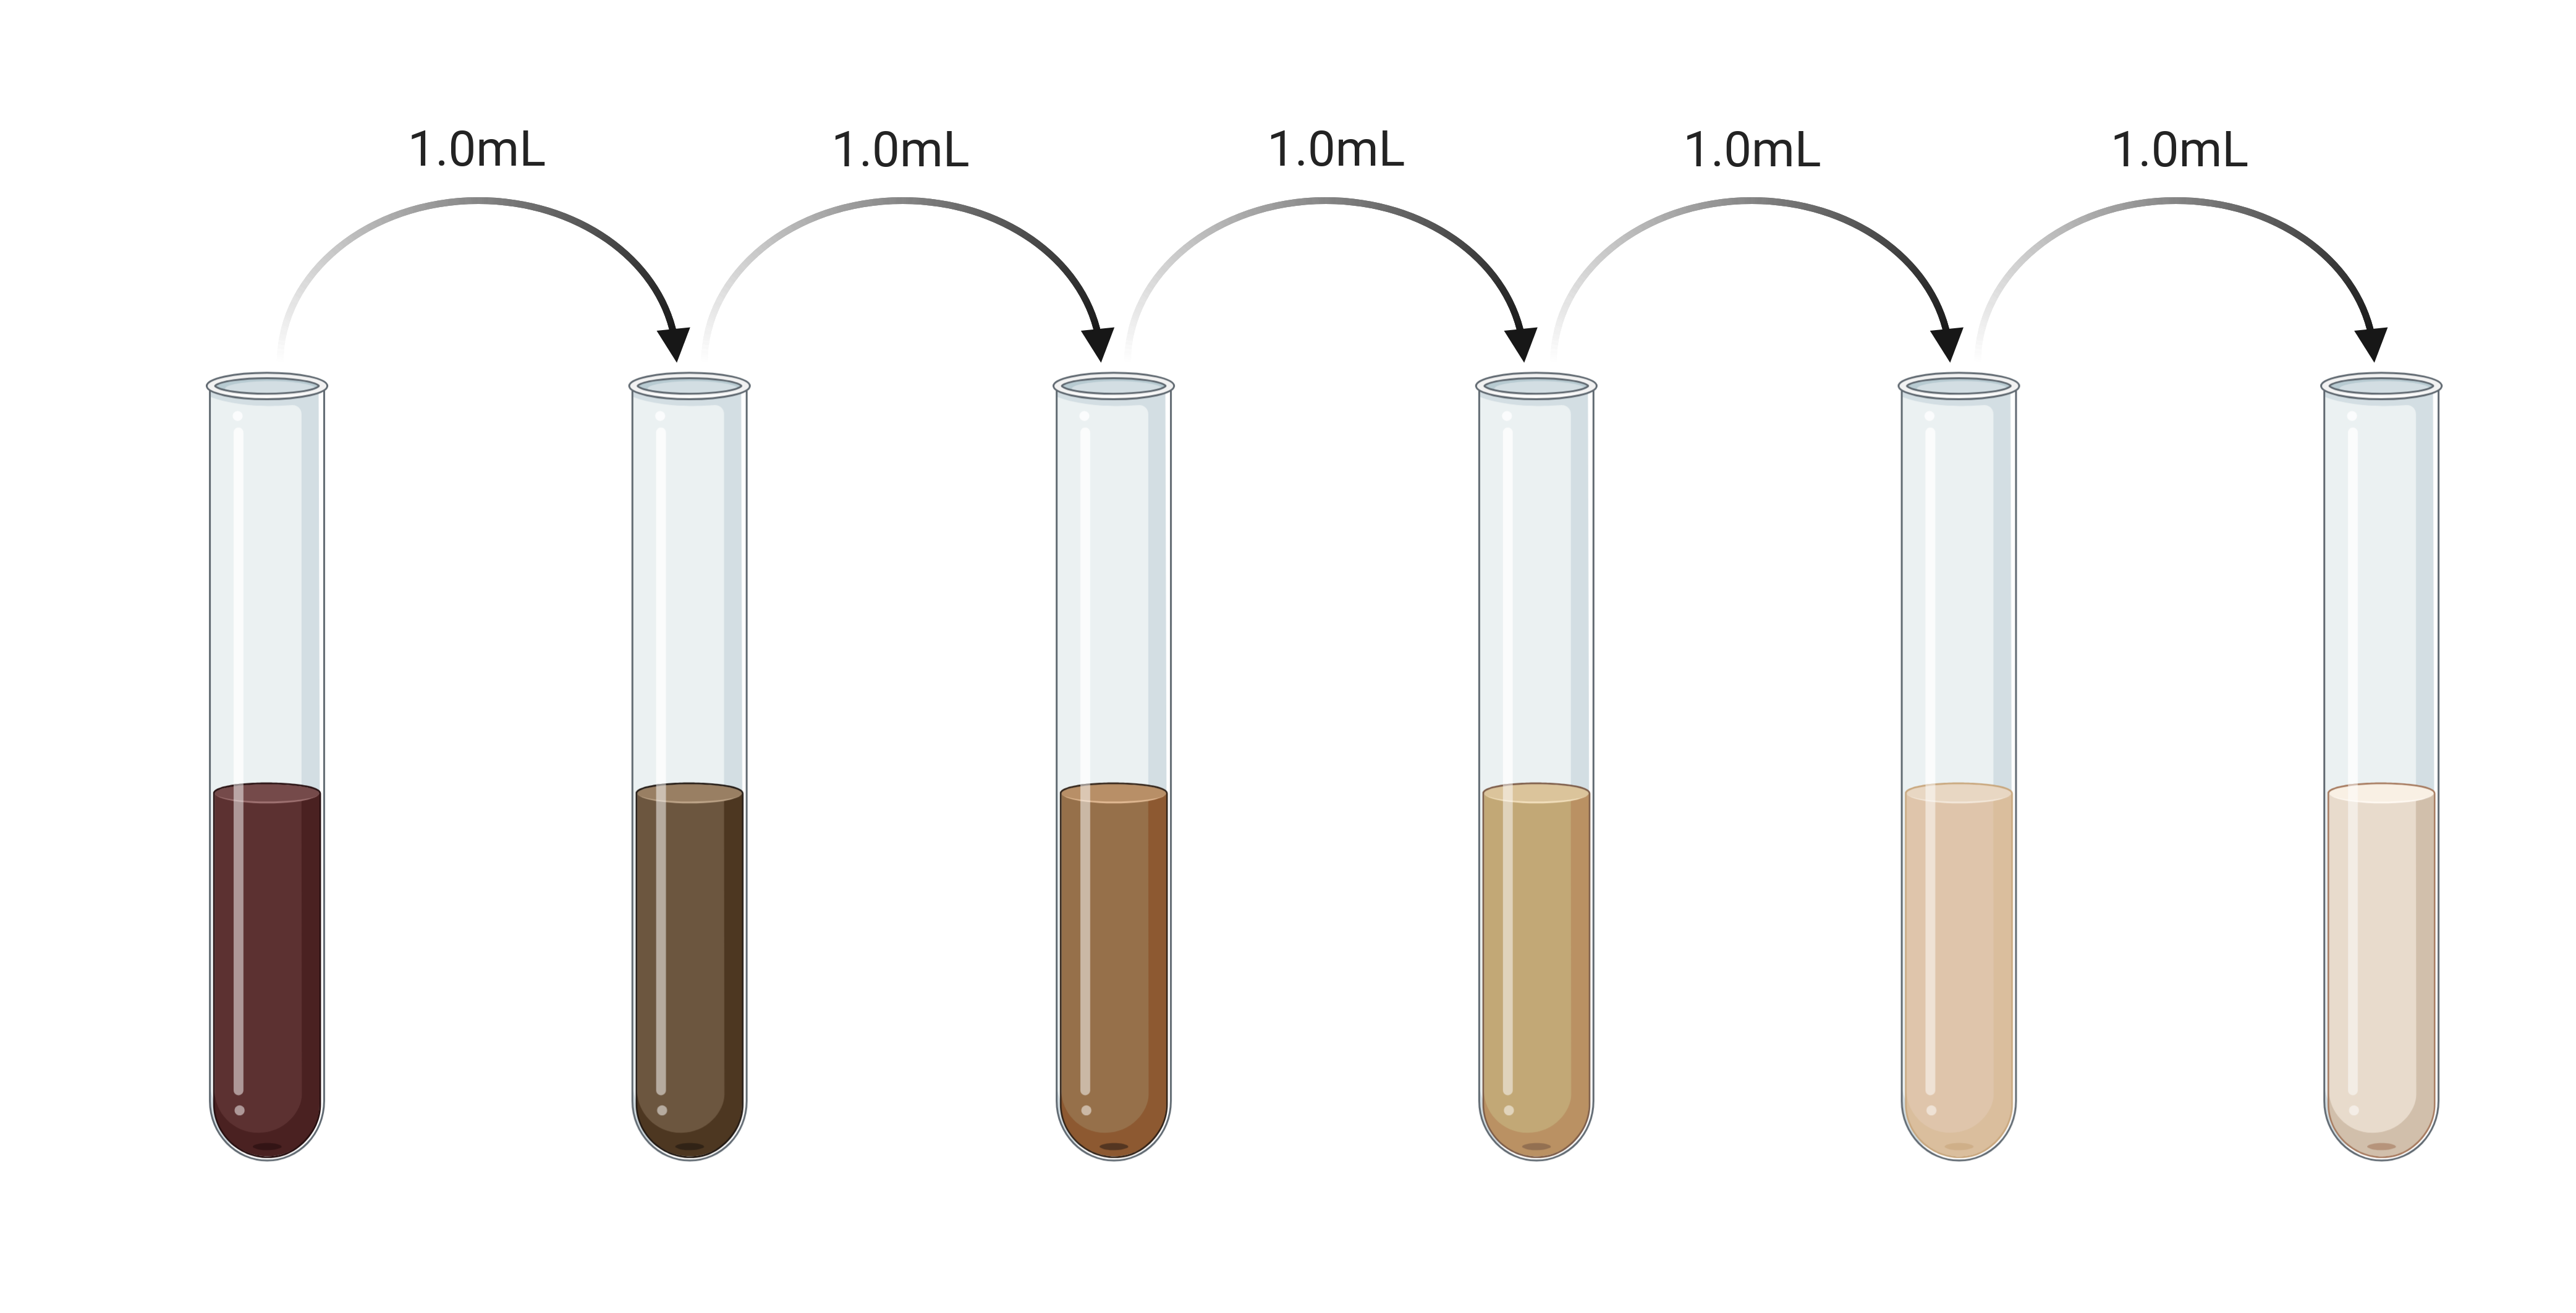
\includegraphics[scale=.3]{FQ/Solucoes/Diluicao.png}
\end{center}
\end{frame}


\begin{frame}[label={sec:orgb9be7e2}]{Exemplo}
\begin{question}
Ao adicionar uma quantia de 75mL de água diretamente em 25mL de uma solução 0,20 \unit{\mol\per\litre} de cloreto de sódio (NaC\(\ell\)), obtemos uma solução de concentração molar igual a:
\end{question}

\begin{answer}[print=true]
Volume adicionado (V\textsubscript{a}) = 75 mL;  Volume inicial (V\textsubscript{i}) = 25 mL; Molaridade inicial (\(\mathcal{M}_i\)) = 0,2 \unit{\mol\per\litre}; Molaridade final (\(\mathcal{M}_f\)) = ?

\begin{align*}
\mathcal{M}_i \cdot V_i = \mathcal{M}_f \cdot V_f \\
0,2 \cdot 25 = \mathcal{M}_f \cdot 100\\
\mathcal{M}_f= 0,05~\unit{\mol\per\litre}
\end{align*}
=======
\begin{center}
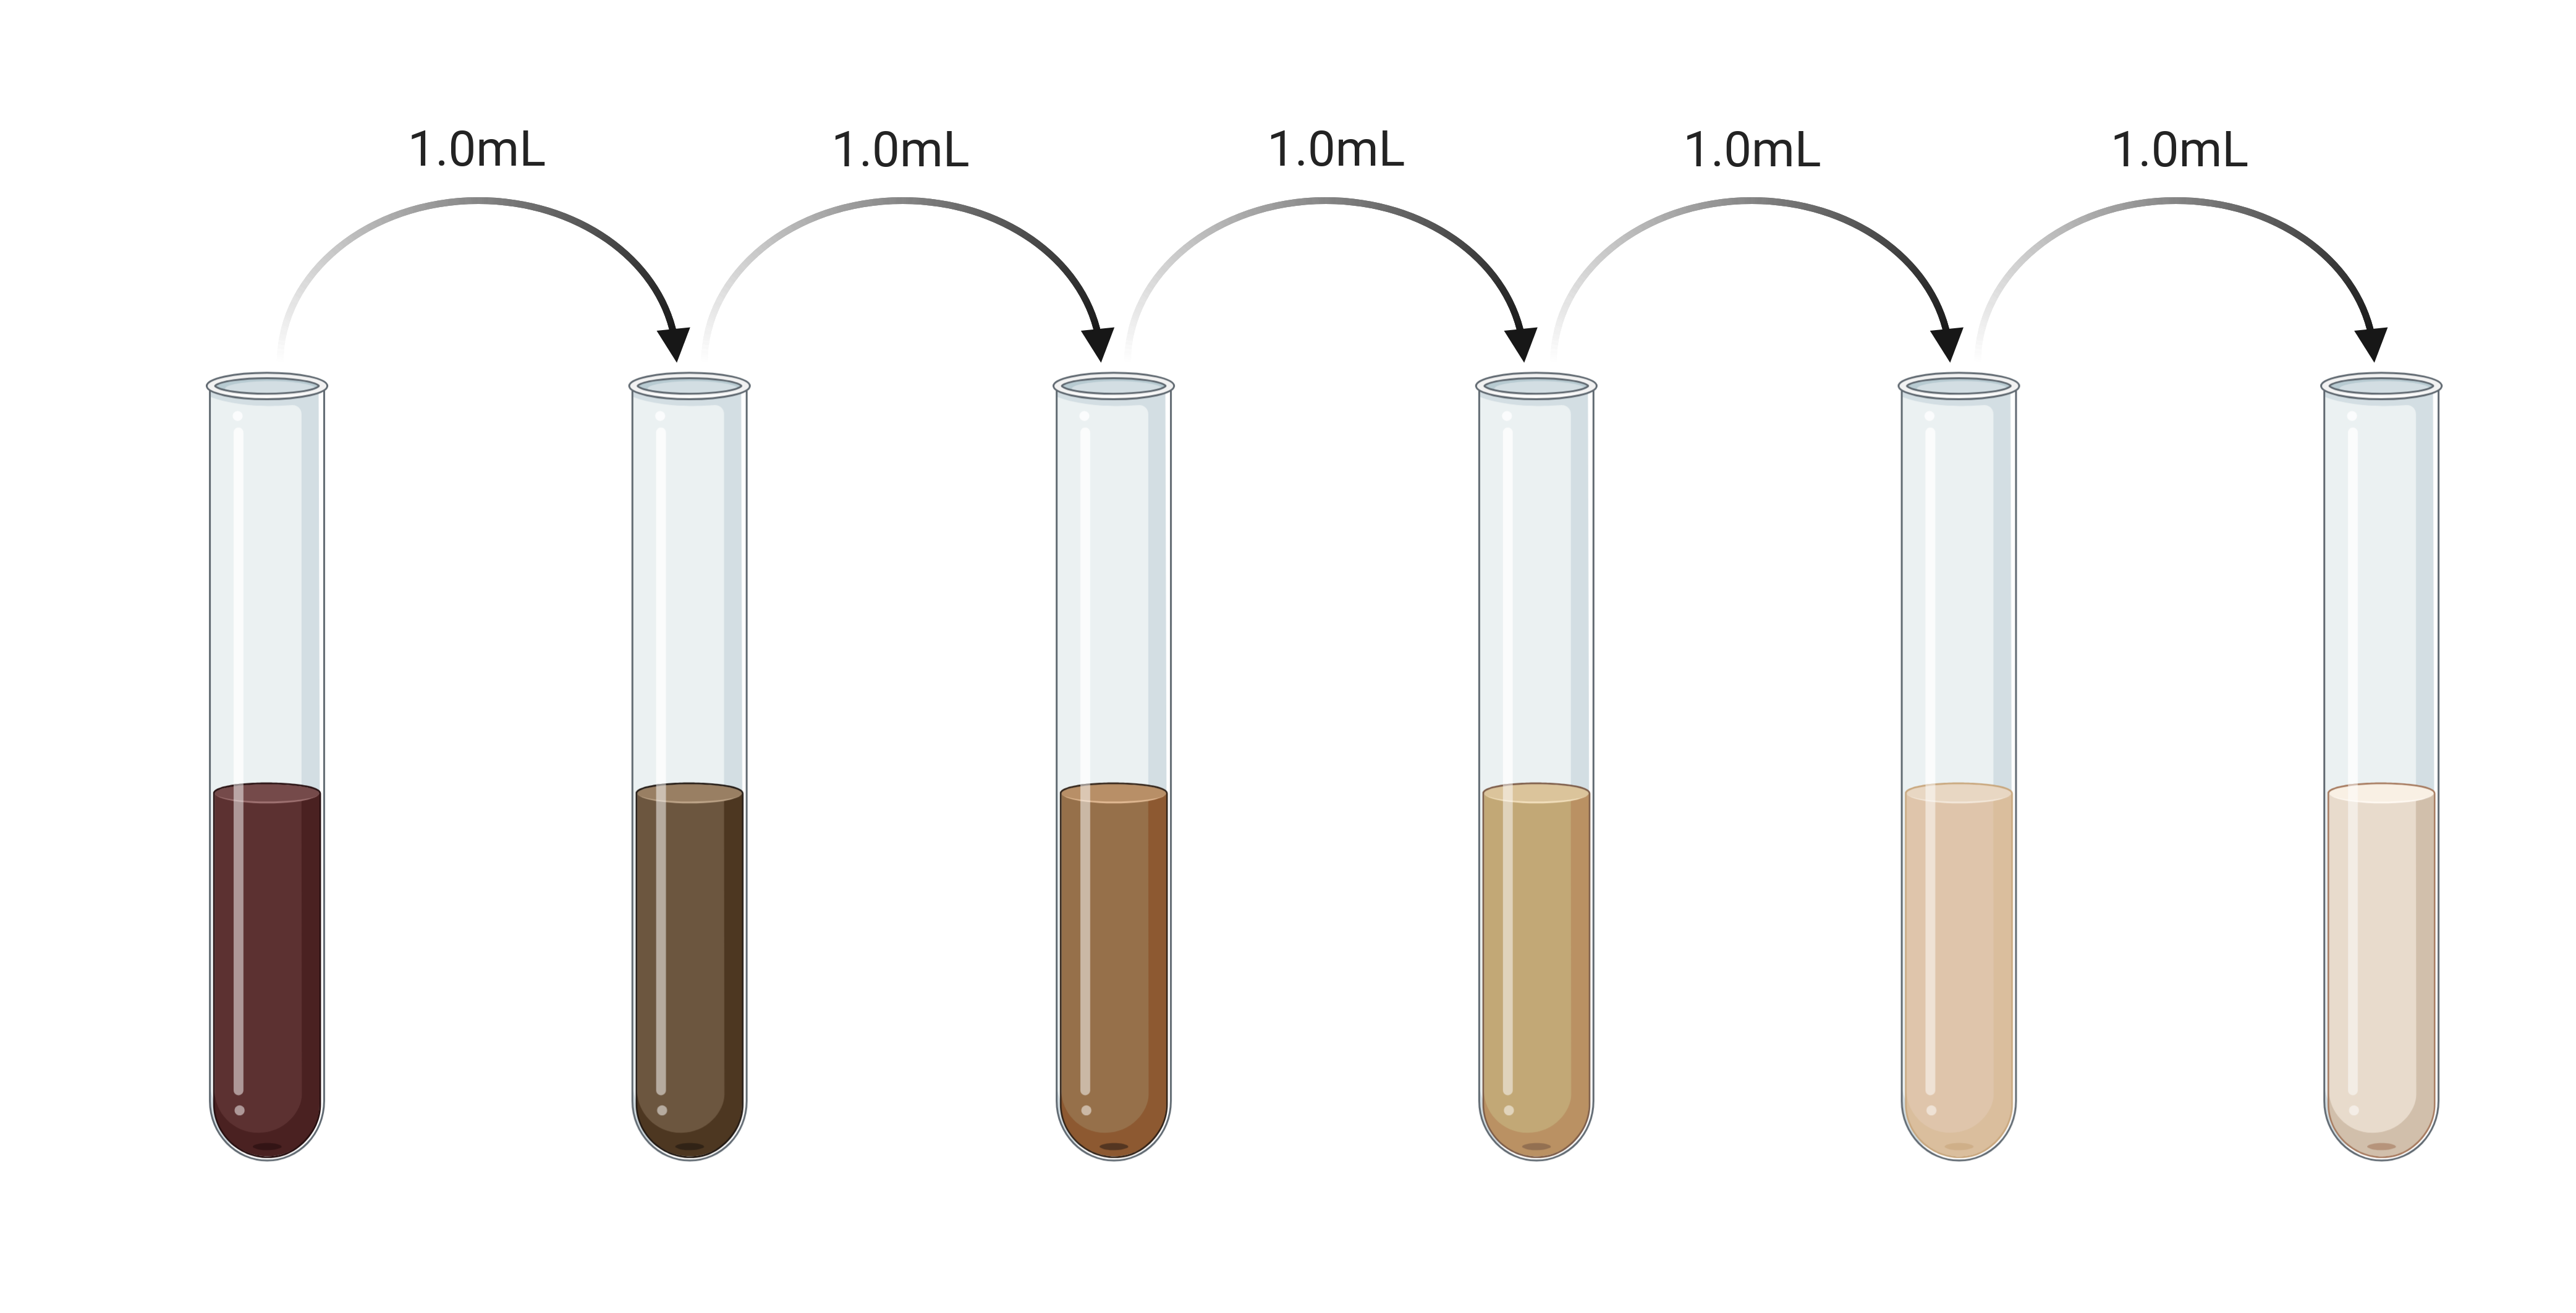
\includegraphics[scale=0.05]{FQ/Solucoes/Diluicao.png}
\end{center}
\end{frame}

\begin{frame}[label={sec:org653554f}]{Exemplo}
\begin{question}
Ao diluir 100 mL de uma solução de concentração igual a 15g/L ao volume final de 150 mL, a nova concentração será?
\end{question}

\begin{answer}[print=true]
\begin{tcolorbox}[ams align*]
\mathcal{M}_1 \cdot V_1 = \mathcal{M}_2 \cdot V_2\\
15 \cdot 100 = \mathcal{M}_2 \cdot 150 \\
\mathcal{M}_2= 1500/150 \\
\mathcal{M}_2 = 10 \; \unit{\gram\per\litre}
\end{tcolorbox}
>>>>>>> 26a94091299b2cda35efc4a2f640ed92afe36773
\end{answer}
\end{frame}

\section{Mistura de Soluções}
<<<<<<< HEAD
\label{sec:org8646531}


\begin{frame}[label={sec:orgfc269cc}]{Mistura de Soluções}
=======
\label{sec:orga628cc8}
\begin{frame}[label={sec:org5e14282}]{Mistura de Soluções}
>>>>>>> 26a94091299b2cda35efc4a2f640ed92afe36773
\begin{itemize}
\item Ocorre quando uma mistura de soluções de mesmo soluto sem reação química consiste em reunir em um mesmo recipiente duas soluções.
\end{itemize}

\begin{tcolorbox}[ams align]
\mathcal{M}_f= \frac{\mathcal{M}_1 \cdot V_1 + \mathcal{M}_2 \cdot V_2}{V_1 + V_2}
\end{tcolorbox}

<<<<<<< HEAD

\begin{center}
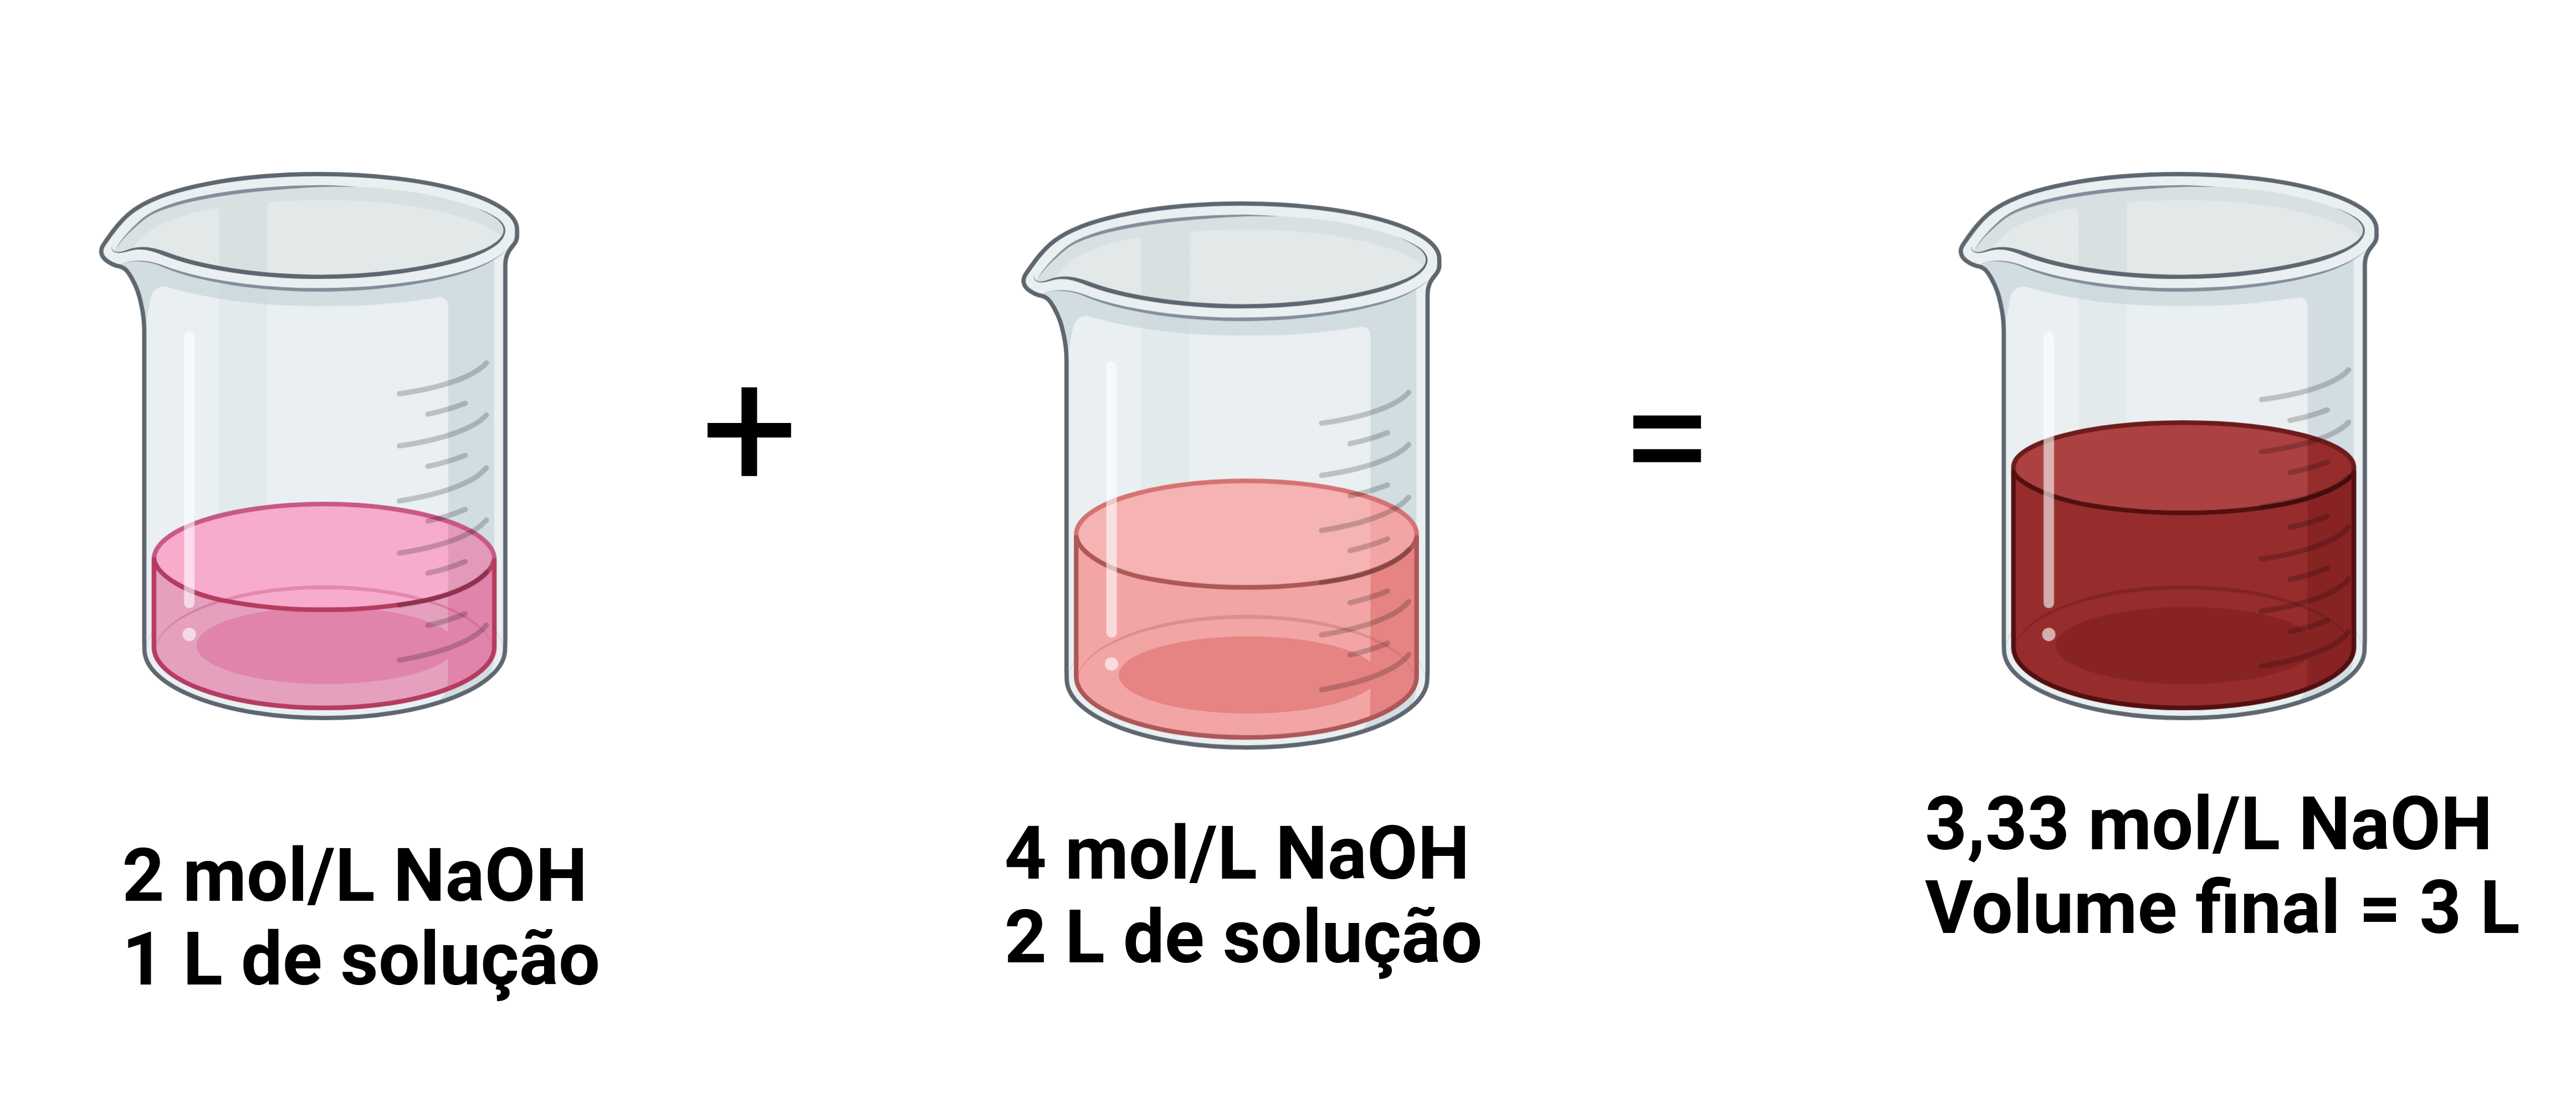
\includegraphics[scale=.3]{FQ/Solucoes/Mistura_Solucao.png}
=======
\begin{center}
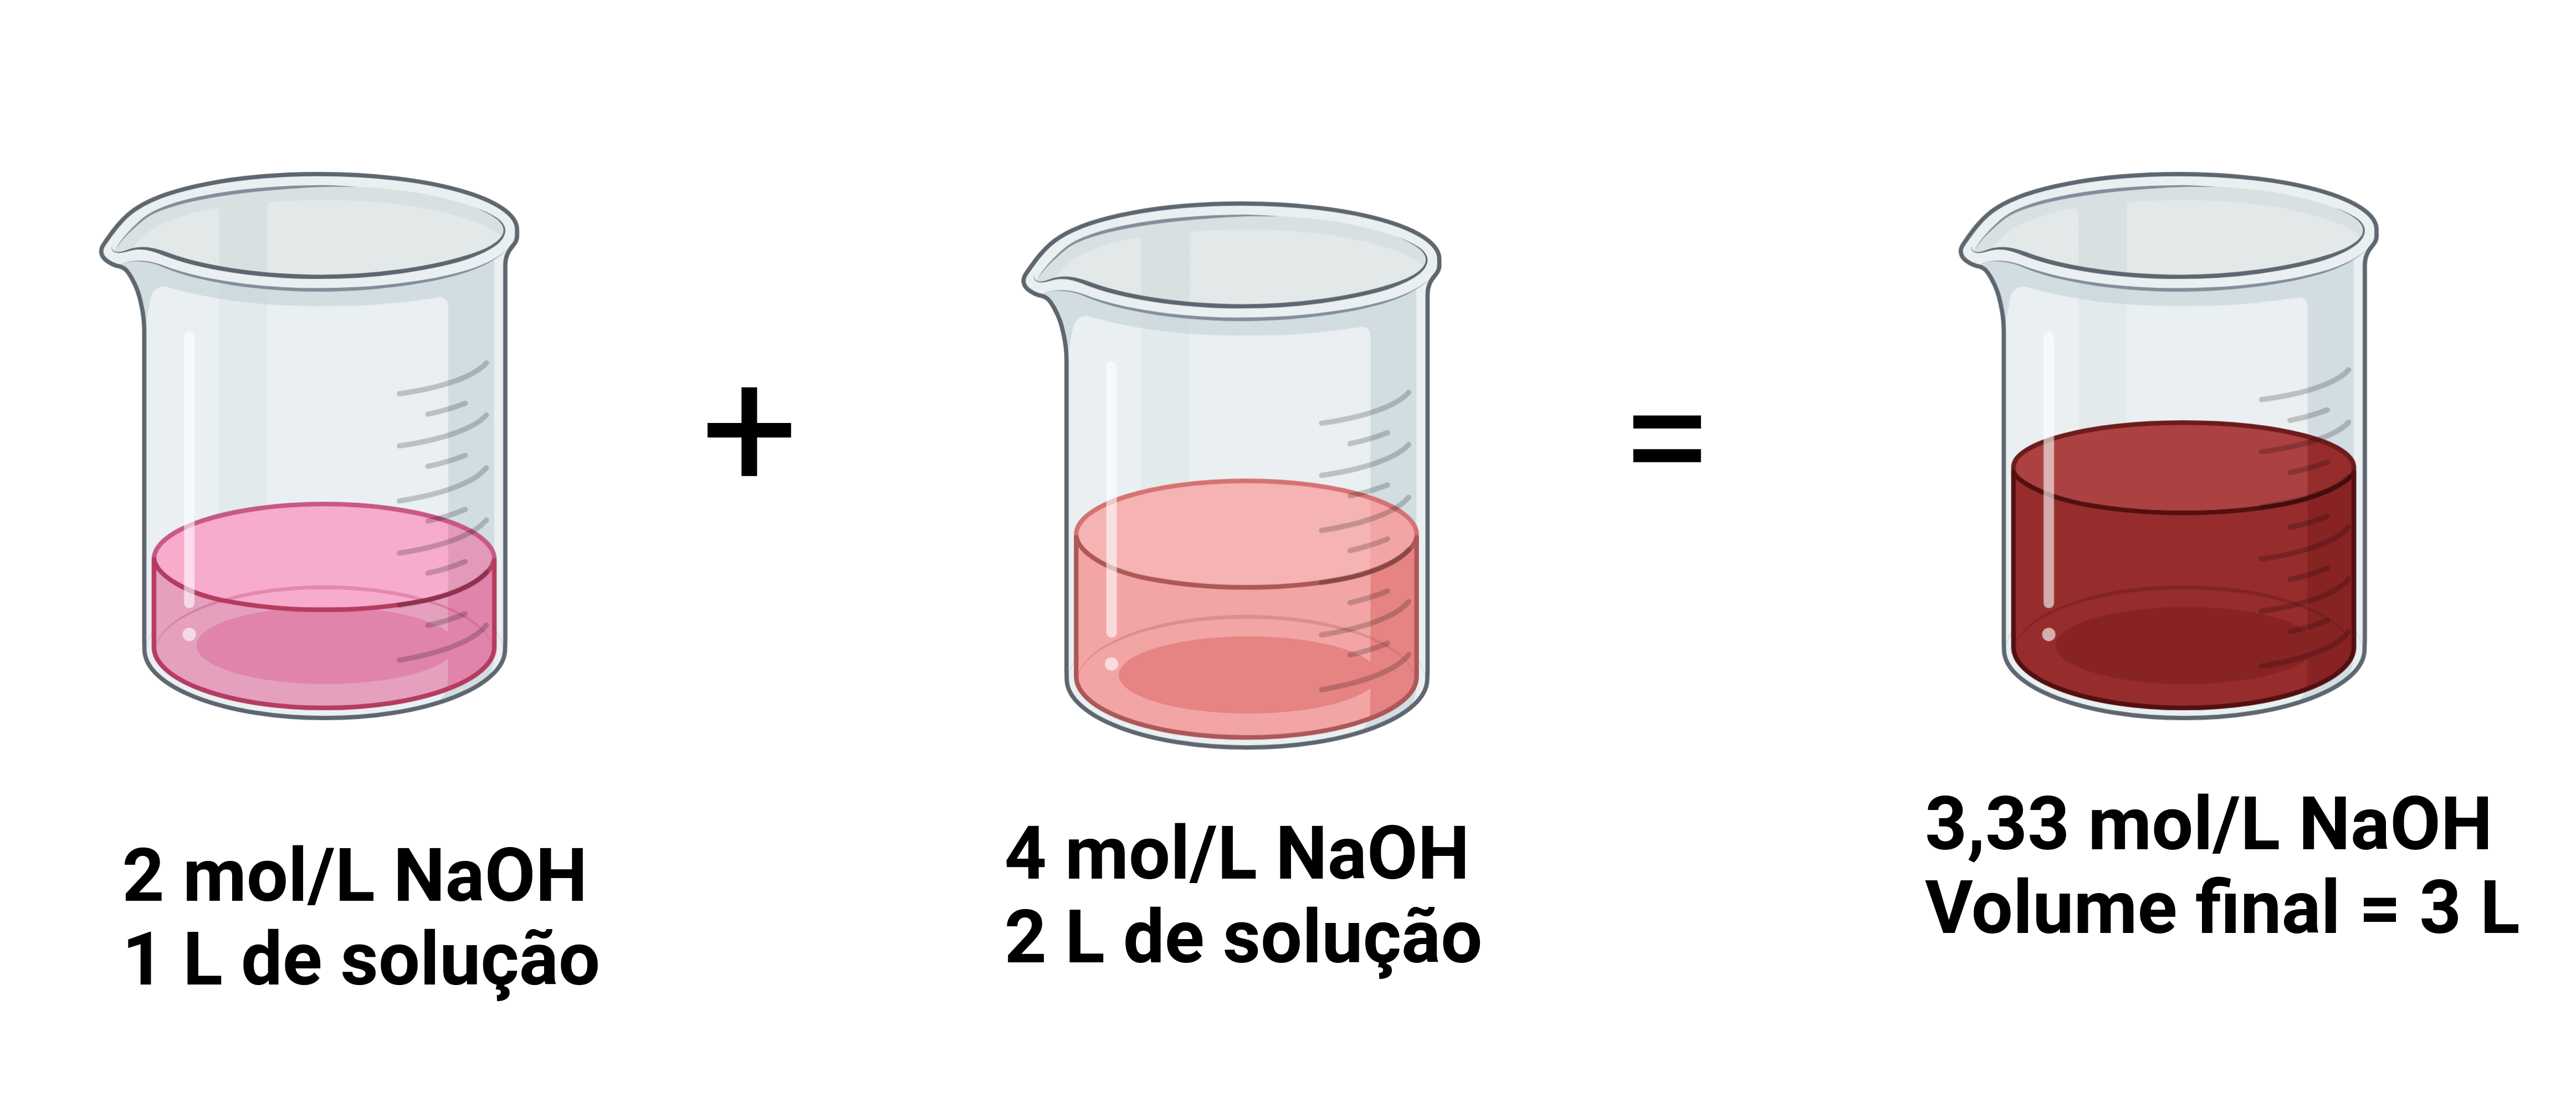
\includegraphics[scale=0.05]{FQ/Solucoes/Mistura_Solucao.png}
>>>>>>> 26a94091299b2cda35efc4a2f640ed92afe36773
\end{center}
\end{frame}



<<<<<<< HEAD

\begin{frame}[label={sec:org4e85eb6}]{Exemplo}
=======
\begin{frame}[label={sec:org5118850}]{Exemplo}
>>>>>>> 26a94091299b2cda35efc4a2f640ed92afe36773
\begin{question}
Se misturarmos 400 mL de uma solução aquosa de NaC\(\ell\) 0,2 mol/L com 250 mL de outra solução de NaC\(\ell\) 0,4 mol/L, teremos uma nova solução. Qual será a concentração em \unit{\mol\per\litre} da solução final?
\end{question}


\begin{answer}[print=true]
\small
\begin{tcolorbox}[ams align*]
\mathcal{M}_f= & \frac{\mathcal{M}_1 \cdot V_1 + \mathcal{M}_2 \cdot V_2}{V_1 + V_2}\\
\mathcal{M}_f= & \frac{0,2 \cdot 400 + 0,4 \cdot 250}{400 + 250}\\
\mathcal{M}_f= & \frac{80+100}{650}\\
\mathcal{M}_f= & 0,27 \unit{\mol\per\litre}
\end{tcolorbox}
\end{answer}
\end{frame}


<<<<<<< HEAD
\begin{frame}[label={sec:org44d85ad}]{Fim da Aula}
=======
\begin{frame}[label={sec:orgb39ec2a}]{Fim da Aula}
>>>>>>> 26a94091299b2cda35efc4a2f640ed92afe36773
\begin{tikzpicture}
\node[graduate,sword, minimum size=1cm]{ \bfseries Bons Estudos !!!!};
\end{tikzpicture}
\begin{center}
\begin{tabular}{ccc}
Download Aula & & \\%Lista de Exercícios
\qrcode[height=2in]{https://github.com/fabinholima/AulaQuimicaPDF/blob/main/FQ/Solucoes.pdf} \\  %\qrcode[height=2in]{https://mark.nl.tab.digital/s/LQwiRJGiybMj32g}\\
 \end{tabular}
 \end{center}
\end{frame}
\end{document}
